\documentclass[11pt,a4paper]{article}

\usepackage[utf8]{inputenc}
\usepackage[T1]{fontenc}
\usepackage{lmodern}
\usepackage[margin=1in]{geometry}
\usepackage{graphicx}
\usepackage{float}
\usepackage{booktabs}
\usepackage{amsmath,amssymb}
\usepackage{tabularx}
\usepackage{microtype}
\usepackage{xcolor}
\usepackage{hyperref}
\usepackage{listings}
\usepackage{tikz}
\usetikzlibrary{shapes.geometric, arrows.meta, positioning, calc, fit, backgrounds}

\hypersetup{
    colorlinks=true,
    linkcolor=blue!70!black,
    citecolor=blue!70!black,
    urlcolor=blue!70!black
}

\lstset{
    basicstyle=\small\ttfamily,
    breaklines=true,
    frame=single,
    numbers=none,
    backgroundcolor=\color{gray!10}
}

\title{
    \textbf{Campus Course Management System (Campus CMS)} \\
    \Large Architecture, Implementation, and Performance Profiling Report
}

\author{
    \textbf{Team Campus CMS} \\
    V Kavyanjali: Dashboard Integration, UI Design System, Synthetic Data Generator \\
    Avani Rohit Kasar: Faculty, Course Management, and Grading \\
    Sahana G Bhagwat: Enrollment Management, Reporting, and Query Profiling \\
    SiriValli: Grading \& Assessment and Integration/Testing
}

\date{\today}

\begin{document}

\maketitle

\begin{abstract}
\noindent\textbf{Problem:} Academic course administration spans student and faculty record-keeping, course scheduling, enrollment approvals, and assessment grading. Handling these workflows in disconnected tools leads to data inconsistencies, duplicate enrollments, unauthorized access, and severe query bottlenecks at institutional scale.

\medskip
\noindent\textbf{Solution:} \textbf{Campus CMS} is a single-semester desktop course management application built with Java 17, Swing (FlatLaf), and SQLite 3. It enforces role-based access control across dedicated \texttt{ADMIN}, \texttt{FACULTY}, and \texttt{STUDENT} portals, separates concerns across DAO, Service, and UI Design System layers, and pairs with Python 3 CLI utilities for deterministic synthetic data generation and query profiling.

\medskip
\noindent\textbf{Major Results:}
\begin{itemize}
    \item \textbf{Scalable Data Synthesis:} Generates 10{,}000+ schema-compliant student accounts with full Java PBKDF2-HMAC-SHA256 password parity in $\sim$40.7 seconds.
    \item \textbf{Query Optimization:} Adding five targeted B-tree indexes on a dataset of 10{,}006 students and 50{,}040 enrollments accelerated \emph{Browse Courses} by \textbf{74$\times$} (146.5\,ms $\rightarrow$ 1.98\,ms) and \emph{CGPA Calculation} by \textbf{100$\times$} (2.51\,ms $\rightarrow$ 0.025\,ms).
    \item \textbf{Verified Reliability:} Passes \textbf{147 automated tests} (136 JUnit 5 tests and 11 Python unit tests) with 0 failures across all modules.
\end{itemize}
\end{abstract}

\tableofcontents
\newpage

\section{Introduction}
\label{sec:introduction}

\subsection{Background and Motivation}
Campus academic administration involves multiple connected activities: maintaining student and faculty records, managing the course catalogue, processing enrollment requests, creating assessments, and recording grades. When these activities are handled separately, it becomes difficult to keep information consistent and provide timely access to students, faculty members, and administrators.

The \textbf{Campus Course Management System (Campus CMS)} is a Java desktop application that organizes these operations around a shared SQLite database. It provides role-specific graphical interfaces for administrators, faculty members, and students, while keeping database access and application rules separate from the user interface.

\subsection{Problem Statement}
A course management application must represent relationships between users, students, faculty members, courses, enrollments, assignments, and grades. It must support common academic workflows without permitting duplicate enrollment records, invalid course data, unauthorized changes, or premature disclosure of draft grades. The project addresses these requirements through a centralized application backed by a relational database.

\subsection{Project Objectives}
The principal objectives are:
\begin{itemize}
    \item Provide login and role-based access for \texttt{ADMIN}, \texttt{FACULTY}, and \texttt{STUDENT} accounts.
    \item Maintain student and faculty profiles, including account and record status.
    \item Support course creation and management, faculty assignment, credits, capacity, semester, and course status.
    \item Enable course browsing, enrollment requests, administrative approval or rejection, and course drops.
    \item Support assignment and quiz records, grade entry, draft grades, and publication of grades.
    \item Provide academic and enrollment reports, including CSV export where supported.
    \item Preserve data integrity using relational constraints and application-level validation.
    \item Evaluate and improve selected database queries using profiling and indexes.
\end{itemize}

\subsection{Scope}
The application is organized around three roles. Administrators manage student and faculty records, course offerings, enrollment decisions, and administrative reports. Faculty members work with their assigned courses, assessments, and grades. Students browse courses, request enrollment, review their course information, and view assignments and published grades.

The current database schema targets a \emph{single-semester} catalogue. Each course has a slot label, and a database constraint prevents two active courses from using the same slot. Slot labels are not mapped to clock times. Although prerequisite and detailed timetable functionality appeared in the initial project plan, the uploaded schema does not contain prerequisite or timetable tables; those features are not claimed as implemented here.

\subsection{Technology Stack}
\begin{itemize}
    \item \textbf{Java 17 and Swing:} desktop application logic and graphical user interface.
    \item \textbf{FlatLaf:} Swing look-and-feel dependency.
    \item \textbf{SQLite and JDBC:} relational data storage and Java database connectivity.
    \item \textbf{Maven:} dependency management, compilation, packaging, and test execution.
    \item \textbf{JUnit 5:} automated Java tests.
    \item \textbf{Python 3:} synthetic data generation, supplementary reporting, and query profiling.
    \item \textbf{Bash:} scripts for setup, building, execution, testing, and profiling.
\end{itemize}

\subsection{High-Level Architecture}
The source code is grouped into authentication, student management, course catalogue, enrollment, grading, reporting, and dashboard packages. Model classes represent domain entities. Data Access Objects (DAOs) encapsulate SQL operations; service classes implement application rules where appropriate; and Swing panels present data and invoke application operations. The shared database component manages connections to SQLite. Figure~\ref{fig:system-architecture} illustrates the four-tier layered architecture of Campus CMS.

\begin{figure}[H]
\centering
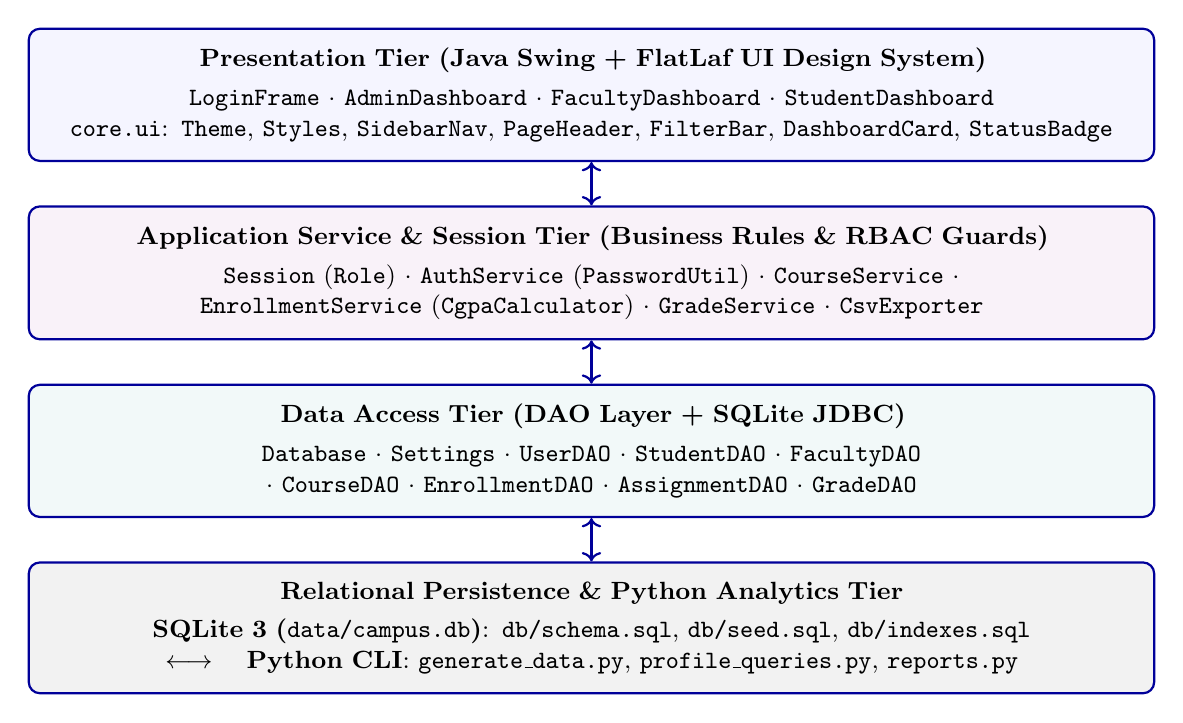
\begin{tikzpicture}[
    node distance=0.55cm,
    tier/.style={rectangle, rounded corners=4pt, draw=blue!60!black, thick, fill=blue!4, text width=13.8cm, align=center, inner sep=7pt, font=\small},
    subbox/.style={rectangle, rounded corners=2pt, draw=gray!70!black, fill=white, inner sep=4pt, font=\footnotesize\ttfamily},
    arrow/.style={-{Stealth[length=2.5mm]}, thick, draw=blue!60!black}
]
    \node[tier] (ui) {
        \textbf{Presentation Tier (Java Swing + FlatLaf UI Design System)}\\[3pt]
        \texttt{LoginFrame} $\cdot$ \texttt{AdminDashboard} $\cdot$ \texttt{FacultyDashboard} $\cdot$ \texttt{StudentDashboard}\\
        \texttt{core.ui}: \texttt{Theme}, \texttt{Styles}, \texttt{SidebarNav}, \texttt{PageHeader}, \texttt{FilterBar}, \texttt{DashboardCard}, \texttt{StatusBadge}
    };

    \node[tier, below=of ui, fill=violet!5!white] (service) {
        \textbf{Application Service \& Session Tier (Business Rules \& RBAC Guards)}\\[3pt]
        \texttt{Session} (\texttt{Role}) $\cdot$ \texttt{AuthService} (\texttt{PasswordUtil}) $\cdot$ \texttt{CourseService} $\cdot$ \texttt{EnrollmentService} (\texttt{CgpaCalculator}) $\cdot$ \texttt{GradeService} $\cdot$ \texttt{CsvExporter}
    };

    \node[tier, below=of service, fill=teal!5!white] (dao) {
        \textbf{Data Access Tier (DAO Layer + SQLite JDBC)}\\[3pt]
        \texttt{Database} $\cdot$ \texttt{Settings} $\cdot$ \texttt{UserDAO} $\cdot$ \texttt{StudentDAO} $\cdot$ \texttt{FacultyDAO} $\cdot$ \texttt{CourseDAO} $\cdot$ \texttt{EnrollmentDAO} $\cdot$ \texttt{AssignmentDAO} $\cdot$ \texttt{GradeDAO}
    };

    \node[tier, below=of dao, fill=gray!10] (db) {
        \textbf{Relational Persistence \& Python Analytics Tier}\\[3pt]
        \textbf{SQLite 3 (\texttt{data/campus.db})}: \texttt{db/schema.sql}, \texttt{db/seed.sql}, \texttt{db/indexes.sql} $\quad\longleftrightarrow\quad$ \textbf{Python CLI}: \texttt{generate\_data.py}, \texttt{profile\_queries.py}, \texttt{reports.py}
    };

    \draw[arrow, <->] (ui.south) -- (service.north);
    \draw[arrow, <->] (service.south) -- (dao.north);
    \draw[arrow, <->] (dao.south) -- (db.north);
\end{tikzpicture}
\caption{Four-tier system architecture of the Campus Course Management System.}
\label{fig:system-architecture}
\end{figure}

\subsection{Report Organization}
The following sections describe the database schema and relationships, the implementation of major application modules, performance profiling, automated testing, and future directions. Together they document the system as implemented in the project repository.


\section{Database Design}
\label{sec:database}

\subsection{Database Overview}
Campus CMS uses \textbf{SQLite} as its relational database, accessed from Java through JDBC. The base database definition is stored in \texttt{db/schema.sql}, sample records are stored in \texttt{db/seed.sql}, and additional performance indexes are defined in \texttt{db/indexes.sql}. The schema is designed for a single semester and contains seven principal tables: \texttt{users}, \texttt{students}, \texttt{faculty}, \texttt{courses}, \texttt{enrollments}, \texttt{assignments}, and \texttt{grades}.

\subsection{Entities and Attributes}
Table~\ref{tab:database-entities} summarizes the seven core tables in the schema along with their primary keys (PK), foreign keys (FK), and principal domain attributes.

\begin{table}[H]
\centering
\small
\begin{tabular}{|p{0.18\linewidth}|p{0.72\linewidth}|}
\hline
\textbf{Table} & \textbf{Important attributes} \\ \hline
\texttt{users} & \texttt{user\_id} (PK), \texttt{username} (unique), \texttt{password\_hash}, \texttt{role}, \texttt{is\_active} \\ \hline
\texttt{students} & \texttt{student\_id} (PK), \texttt{user\_id} (FK, unique), \texttt{roll\_number} (unique), \texttt{name}, \texttt{branch}, \texttt{year}, \texttt{email}, \texttt{status} \\ \hline
\texttt{faculty} & \texttt{faculty\_id} (PK), \texttt{user\_id} (FK, unique), \texttt{name}, \texttt{department}, \texttt{email}, \texttt{status} \\ \hline
\texttt{courses} & \texttt{course\_id} (PK), \texttt{code} (unique), \texttt{title}, \texttt{credits}, \texttt{capacity}, \texttt{semester}, \texttt{slot}, \texttt{faculty\_id} (FK, nullable), \texttt{status} \\ \hline
\texttt{enrollments} & \texttt{enrollment\_id} (PK), \texttt{student\_id} (FK), \texttt{course\_id} (FK), \texttt{status}, \texttt{request\_date} \\ \hline
\texttt{assignments} & \texttt{assignment\_id} (PK), \texttt{course\_id} (FK), \texttt{title}, \texttt{type}, \texttt{description}, \texttt{due\_date}, \texttt{max\_marks}, \texttt{weight}, \texttt{status}, \texttt{material\_path} \\ \hline
\texttt{grades} & \texttt{grade\_id} (PK), \texttt{assignment\_id} (FK), \texttt{student\_id} (FK), \texttt{marks}, \texttt{feedback}, \texttt{published} \\ \hline
\end{tabular}
\caption{Core database tables and attributes. PK denotes primary key; FK denotes foreign key.}
\label{tab:database-entities}
\end{table}

\subsection{Entity Relationships}
A \texttt{users} record may have a corresponding \texttt{students} or \texttt{faculty} profile, linked by a unique foreign key. Administrator accounts need only a \texttt{users} record. One faculty member may be assigned to multiple courses, whereas each course has at most one assigned faculty member; the \texttt{faculty\_id} field may be null until assignment.

Students and courses have a many-to-many relationship represented by \texttt{enrollments}. A course has multiple assignments or quizzes, and each assignment can have grade records for multiple students. The \texttt{grades} table also links each grade to the corresponding student. The pair \texttt{(student\_id, course\_id)} is unique in \texttt{enrollments}; the pair \texttt{(assignment\_id, student\_id)} is unique in \texttt{grades}. Figure~\ref{fig:er-diagram} presents the complete Entity-Relationship (ER) diagram of the database schema.

\begin{figure}[H]
\centering
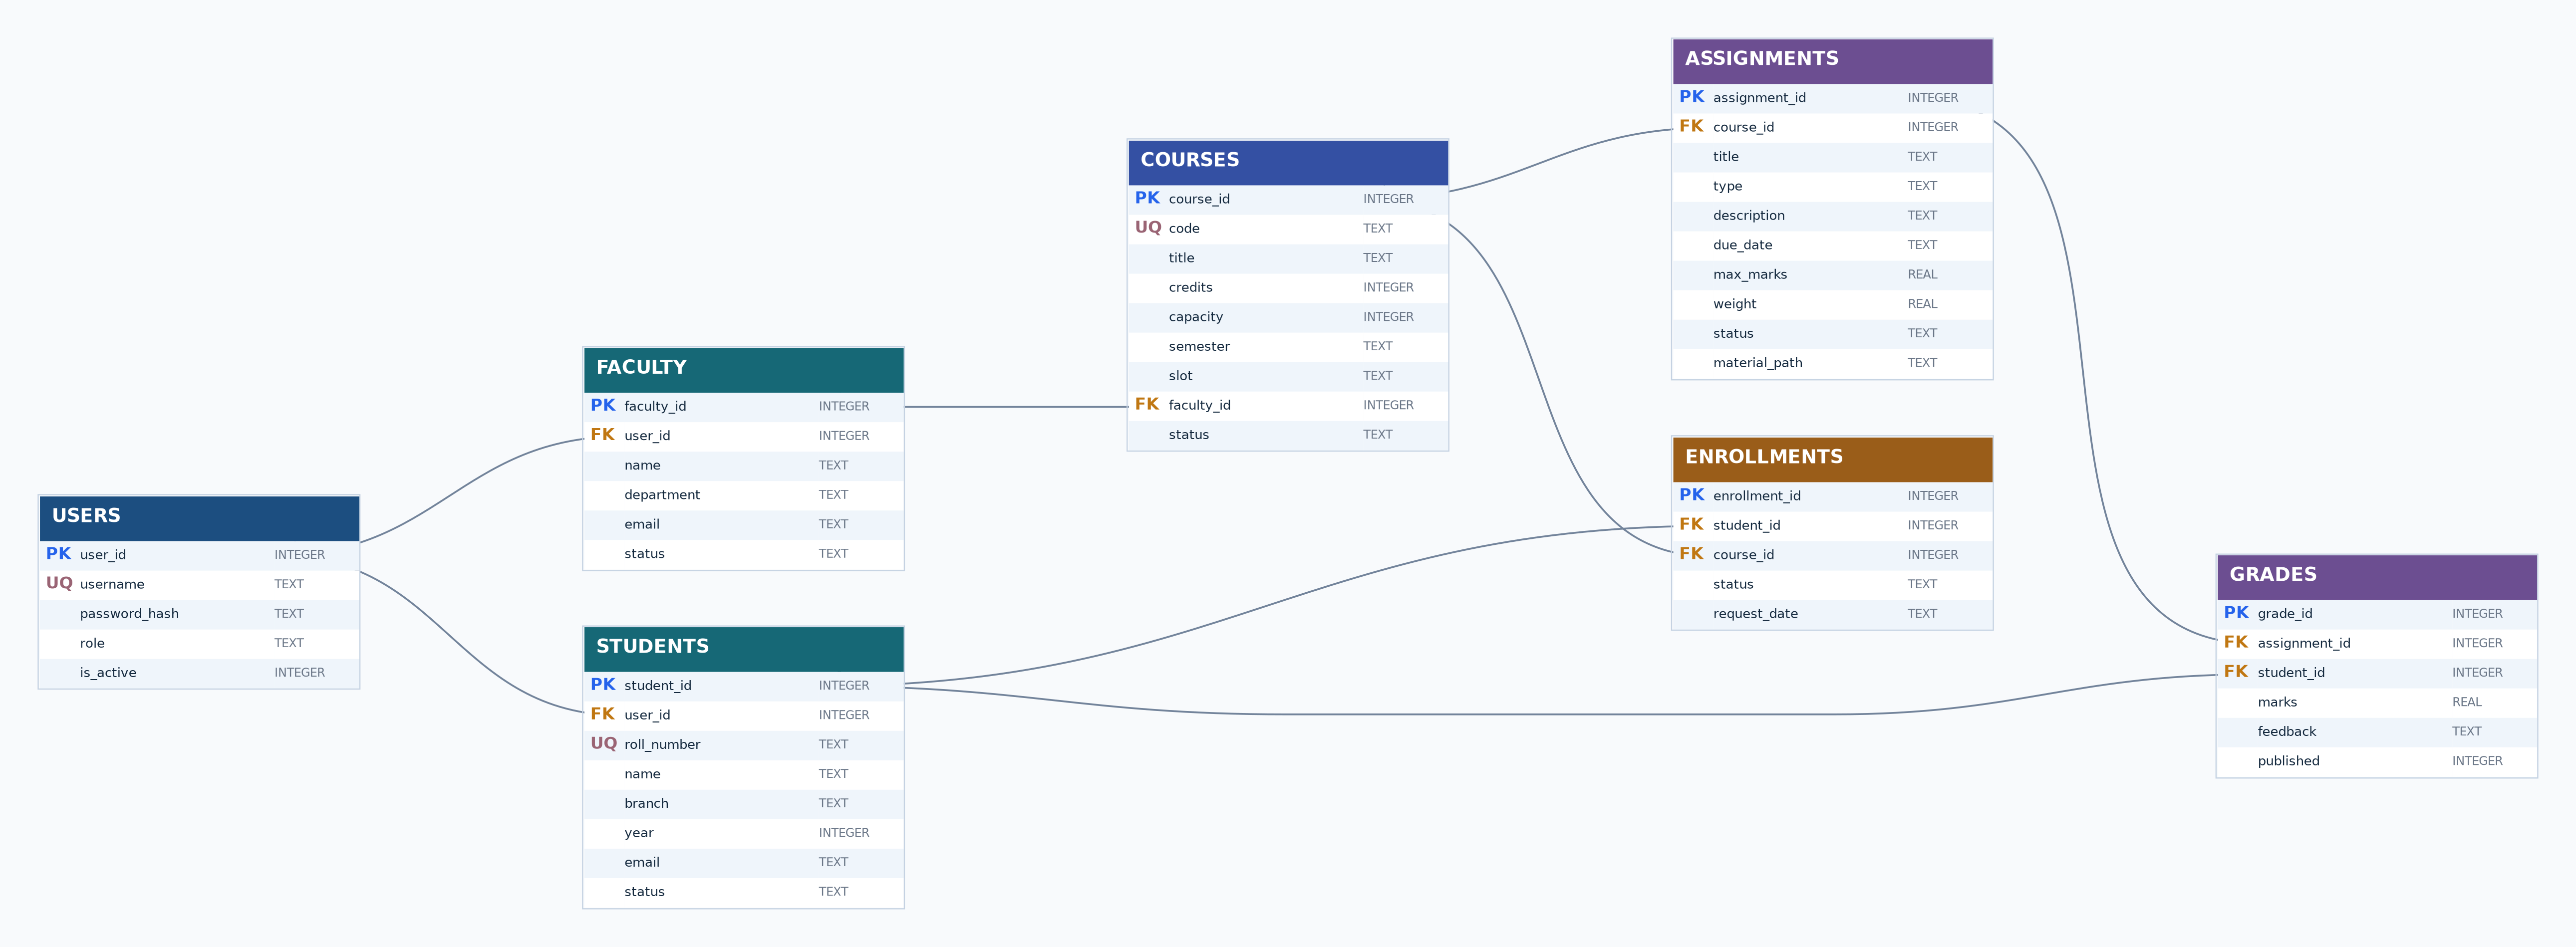
\includegraphics[width=0.92\linewidth]{figures/er_diagram.png}
\caption{Entity-Relationship (ER) diagram of the Campus CMS database schema.}
\label{fig:er-diagram}
\end{figure}

\subsection{Schema Constraints}
\subsubsection{Account and Profile Constraints}
The \texttt{users.role} column accepts only \texttt{ADMIN}, \texttt{FACULTY}, or \texttt{STUDENT}. The \texttt{is\_active} field is restricted to 0 or 1. Student and faculty statuses are restricted to \texttt{ACTIVE} or \texttt{INACTIVE}. Student year must be between 1 and 6. Usernames and student roll numbers must be unique.

\subsubsection{Course Constraints}
Course codes are unique, and credits and capacity must be positive integers. A course is either \texttt{ACTIVE} or \texttt{ARCHIVED}. Every course has a nonempty, trimmed, uppercase \texttt{slot} label. The partial unique index \texttt{idx\_courses\_unique\_active\_slot} prevents two \texttt{ACTIVE} courses from sharing a slot, while allowing archived courses to retain previously used labels. The schema does not represent actual meeting times or prerequisites.

\subsubsection{Enrollment Constraints}
Enrollment status must be one of \texttt{PENDING}, \texttt{APPROVED}, \texttt{REJECTED}, \texttt{DROPPED}, or \texttt{COMPLETED}. New records default to \texttt{PENDING}, with \texttt{request\_date} defaulting to the current date. A student-course pair can occur only once; a dropped enrollment can therefore be reactivated by updating its existing record instead of inserting a duplicate. Course-capacity checks and role permissions are implemented in application logic rather than as database \texttt{CHECK} constraints.

\subsubsection{Assignment and Grade Constraints}
Assignments have type \texttt{ASSIGNMENT} or \texttt{QUIZ}, positive maximum marks, and a weight between 0 and 100. Assignment status is \texttt{OPEN} or \texttt{CLOSED}; due dates are stored as ISO date strings. Grades must have nonnegative marks and a Boolean \texttt{published} flag. Draft grades have \texttt{published = 0}; published grades have \texttt{published = 1}. The application must verify that entered marks do not exceed the associated assignment's maximum, since a row-level SQLite \texttt{CHECK} constraint cannot compare values across these tables.

\subsection{Foreign Keys and Referential Integrity}
The schema defines foreign keys from \texttt{students} and \texttt{faculty} to \texttt{users}; from \texttt{courses} to \texttt{faculty}; from \texttt{enrollments} to \texttt{students} and \texttt{courses}; from \texttt{assignments} to \texttt{courses}; and from \texttt{grades} to \texttt{assignments} and \texttt{students}. SQLite foreign-key enforcement is enabled by \texttt{PRAGMA foreign\_keys = ON}; this setting must also be enabled for each database connection.

\subsection{Indexes and Query Optimization}
The schema automatically obtains indexes for primary keys and unique constraints. It also defines the partial unique active-course slot index. Five additional indexes are maintained in \texttt{db/indexes.sql} for profiling-based optimization:
\begin{itemize}
    \item \texttt{idx\_enrollments\_course\_status} on \texttt{enrollments(course\_id, status)} for course-level enrollment counts, rosters, and approvals.
    \item \texttt{idx\_enrollments\_status} on \texttt{enrollments(status)} for administrative status counts and filtering.
    \item \texttt{idx\_grades\_student} on \texttt{grades(student\_id)} for student-grade retrieval and CGPA calculations.
    \item \texttt{idx\_assignments\_course} on \texttt{assignments(course\_id)} for course-level grade reports and transcript joins.
    \item \texttt{idx\_students\_name} on \texttt{students(name COLLATE NOCASE)} for case-insensitive name-prefix searches.
\end{itemize}
These indexes are kept separate from the base schema so that query timings can be compared before and after optimization. The measurements and trade-offs are presented in the profiling section.

\subsection{Database Setup and Maintenance}
The repository provides \texttt{scripts/setup.sh} to create the database and load seed records. From the project root, the setup command is:
\begin{verbatim}
bash scripts/setup.sh
\end{verbatim}
By default, this creates \texttt{data/campus.db}. The script uses the \texttt{sqlite3} command-line tool if available, or Python's \texttt{sqlite3} module otherwise. Running the setup script replaces the existing local database and reloads the demonstration data. Because the schema intentionally recreates the tables, setup should not be used to preserve production records.

\subsection{Design Considerations}
The design separates login identities from student and faculty profiles, models many-to-many course enrollment through a junction table, and uses foreign keys to maintain relationships. Calculated values such as remaining seats and student CGPA are not stored as redundant columns; they are derived from enrollment and grade data. Database constraints protect record-level consistency, while application services handle workflow rules and authorization. The resulting design is appropriate for the implemented single-semester desktop application and can be extended if detailed timetable, prerequisite, or multi-semester support is introduced later.


\section{Dashboard Architecture and UI Design System}
\label{sec:ui-design-system}

\subsection{Design Language and Philosophy}
To modernize the desktop user experience and eliminate dated Swing aesthetics, a custom design system was implemented within the \texttt{com.campus.cms.core.ui} package. The design language adopts an ``Academic SaaS'' aesthetic inspired by modern enterprise web applications, leveraging the \textbf{FlatLaf} look-and-feel library while establishing a consistent token-driven UI layer.

The visual system centers around:
\begin{itemize}
    \item \textbf{Color Palette:} An authoritative Indigo primary accent (\texttt{\#4F46E5}), deep slate text (\texttt{\#0F172A}), muted gray borders (\texttt{\#E2E8F0}), and light neutral backgrounds (\texttt{\#F4F6FA} for workspace canvases, \texttt{\#FFFFFF} for cards and panels).
    \item \textbf{Typography:} System font scaling with explicit hierarchy: Display Header (22pt bold), Section Titles (16pt bold), Card Subtitles (12pt regular), and Body text (13pt regular).
    \item \textbf{Spatial Metrics and Elevation:} Consistent 8pt grid metrics (spacings of 4, 8, 12, 16, 24, and 32 pixels), subtle border radii (8px for buttons and badges, 12px for cards), and 1px borders rather than heavy bevels.
\end{itemize}

\subsection{Reusable Component Architecture}
The UI design system provides seven core reusable components:
\begin{enumerate}
    \item \textbf{\texttt{Theme.java}:} Central source of truth for color constants, font tokens, borders, and dimensions.
    \item \textbf{\texttt{Styles.java}:} Factory utility providing standardized button variants (\texttt{primary}, \texttt{secondary}, \texttt{destructive}), uniform table formatting with custom header renderers, scroll panes, text input styling, and action bars.
    \item \textbf{\texttt{SidebarNav.java}:} Persistent navigation rail pinned to the left edge of all role portals. Features an institution brand banner, a personalized user avatar chip displaying the user's initials, active navigation pill tracking, and a pinned bottom logout button that safely clears sessions.
    \item \textbf{\texttt{PageHeader.java}:} Standardized header component displaying a prominent section title with a descriptive muted subtitle across all dashboard views.
    \item \textbf{\texttt{FilterBar.java} and \texttt{WrapLayout}:} A responsive filter toolbar component utilizing a custom flow layout that dynamically computes preferred height when filter fields wrap on narrow screens.
    \item \textbf{\texttt{DashboardCard.java}:} Key performance indicator (KPI) metric cards featuring a 4px colored accent stripe (blue, emerald, red, amber, purple), large metric figures, descriptive subtitles, and subtle mouse-hover elevation feedback.
    \item \textbf{\texttt{StatusBadge.java}:} Rounded pill badge component and table cell renderer for displaying entity statuses (e.g., \texttt{ACTIVE}, \texttt{INACTIVE}, \texttt{PENDING}, \texttt{APPROVED}) with semantically appropriate background and text tints.
\end{enumerate}

\subsection{Role-Based Dashboard Implementations}
The application provides three synchronized, role-guarded portal dashboards (shown in Figures~\ref{fig:admin-dashboard}, \ref{fig:faculty-dashboard}, and \ref{fig:student-dashboard}):
\begin{itemize}
    \item \textbf{\texttt{AdminDashboard}:} Provides institutional oversight. Summarizes total, active, and inactive student accounts via \texttt{DashboardCard} widgets. Features a dynamic Quick Access action bar allowing administrators to quickly navigate between Student Management, Enrollment Management, Faculty Management, and Course Offerings without nested menus.
    \item \textbf{\texttt{FacultyDashboard}:} Tailored for teaching staff. Displays assigned course load and student counts. Embeds the course roster, assessment management, and the grading interface.
    \item \textbf{\texttt{StudentDashboard}:} Student portal displaying enrolled course counts, upcoming assignments, published grades, and real-time CGPA calculation. Features course browsing, enrollment tracking, and profile management.
\end{itemize}

\begin{figure}[H]
\centering
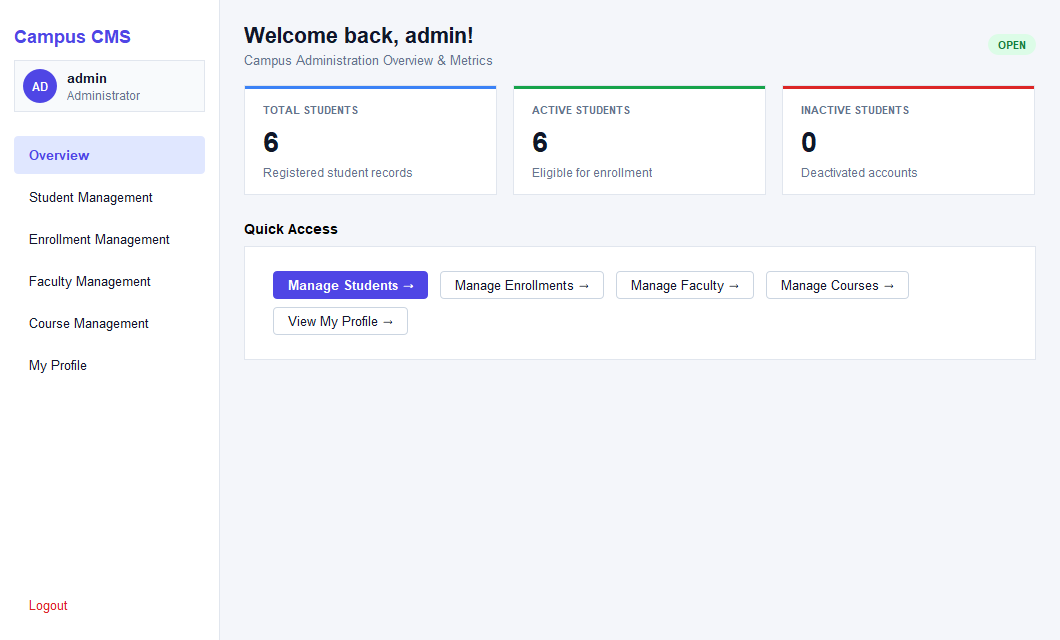
\includegraphics[width=0.92\linewidth]{figures/admin_dashboard.png}
\caption{Administrator Portal (\texttt{AdminDashboard}) displaying KPI metric cards, enrollment period status badge, and wrapped Quick Access action bar.}
\label{fig:admin-dashboard}
\end{figure}

\begin{figure}[H]
\centering
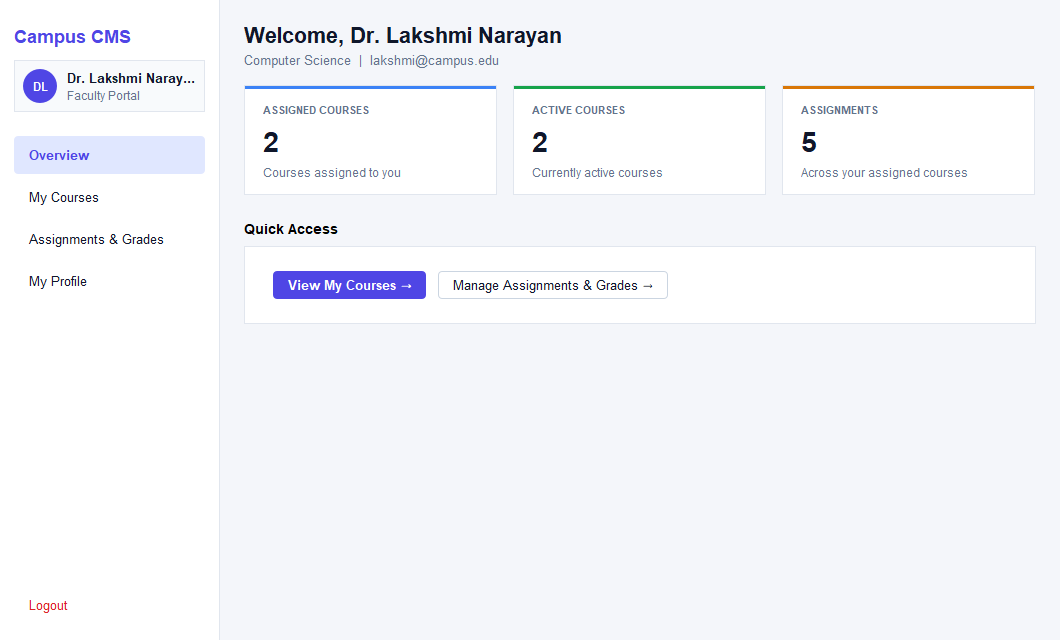
\includegraphics[width=0.92\linewidth]{figures/faculty_dashboard.png}
\caption{Faculty Portal (\texttt{FacultyDashboard}) showing personalized avatar chip, assigned course metrics, and assessment summary.}
\label{fig:faculty-dashboard}
\end{figure}

\begin{figure}[H]
\centering
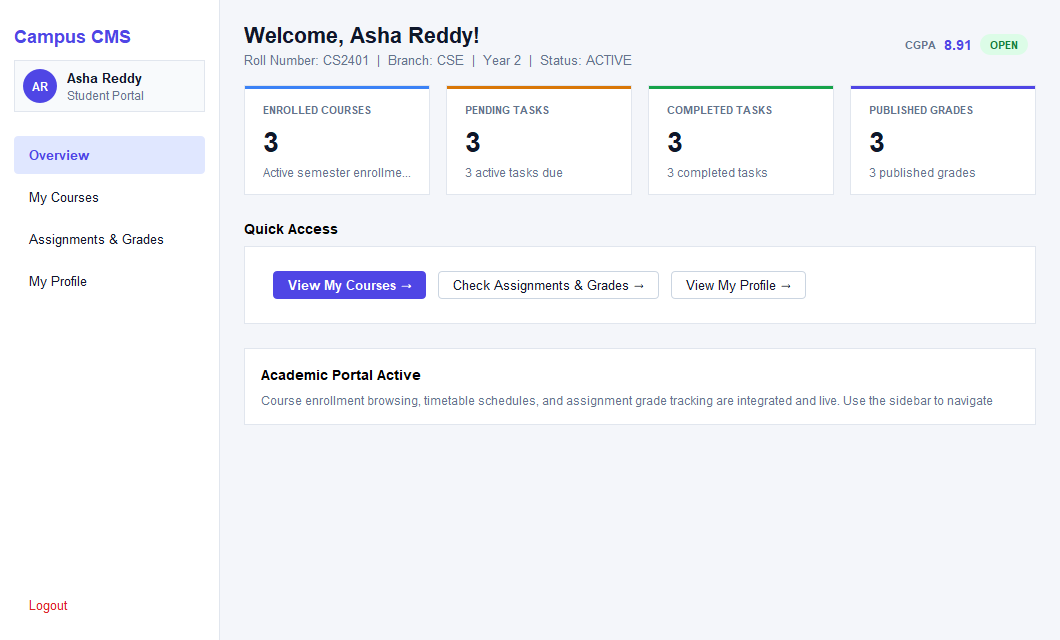
\includegraphics[width=0.92\linewidth]{figures/student_dashboard.png}
\caption{Student Portal (\texttt{StudentDashboard}) showing live CGPA badge, course/task KPI cards, and Quick Access navigation.}
\label{fig:student-dashboard}
\end{figure}

\subsection{Responsive Layout and Action Bar Optimization}
During testing across varied display resolutions, traditional single-line toolbars caused button truncation. To eliminate this issue, \texttt{Styles.actionBar()} was introduced using a multi-row \texttt{WrapLayout}. Unlike standard \texttt{FlowLayout}, \texttt{WrapLayout} dynamically reports its preferred height based on the available width of the parent container, ensuring all action buttons remain fully visible and clickable without horizontal scrollbars or clipping.

\section{Synthetic Student Data Generator}
\label{sec:synthetic-data}

\subsection{Purpose and Motivation}
Realistic performance evaluation of course enrollment systems requires testing at institutional scale (10{,}000+ students). Creating such volumes manually or relying on minimal test fixtures is infeasible. A standalone, high-performance synthetic data generator was developed in Python (\texttt{python/generate\_data.py}) capable of synthesizing realistic student cohorts while ensuring strict database integrity. Figure~\ref{fig:generator-workflow} depicts the end-to-end execution workflow of the synthetic data generator.

\begin{figure}[H]
\centering
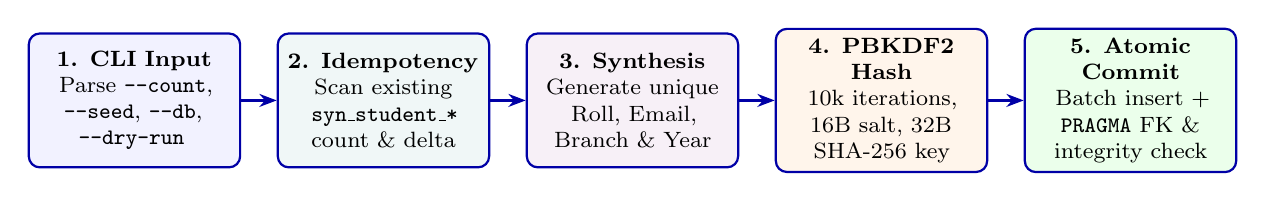
\begin{tikzpicture}[
    node distance=0.45cm,
    stage/.style={rectangle, rounded corners=4pt, draw=blue!65!black, thick, fill=blue!5, text width=2.45cm, minimum height=1.7cm, align=center, font=\footnotesize},
    arrow/.style={-{Stealth[length=2.2mm]}, thick, draw=blue!65!black}
]
    \node[stage] (cli) {\textbf{1. CLI Input}\\Parse \texttt{--count}, \texttt{--seed}, \texttt{--db}, \texttt{--dry-run}};
    \node[stage, right=of cli, fill=teal!6] (idem) {\textbf{2. Idempotency}\\Scan existing \texttt{syn\_student\_*} count \& delta};
    \node[stage, right=of idem, fill=violet!6] (synth) {\textbf{3. Synthesis}\\Generate unique Roll, Email, Branch \& Year};
    \node[stage, right=of synth, fill=orange!8] (hash) {\textbf{4. PBKDF2 Hash}\\10k iterations, 16B salt, 32B SHA-256 key};
    \node[stage, right=of hash, fill=green!8] (tx) {\textbf{5. Atomic Commit}\\Batch insert + \texttt{PRAGMA} FK \& integrity check};

    \draw[arrow] (cli) -- (idem);
    \draw[arrow] (idem) -- (synth);
    \draw[arrow] (synth) -- (hash);
    \draw[arrow] (hash) -- (tx);
\end{tikzpicture}
\caption{Five-stage execution workflow of the synthetic student data generator (\texttt{python/generate\_data.py}).}
\label{fig:generator-workflow}
\end{figure}

\subsection{Architecture and Schema Compliance}
The generator directly interfaces with SQLite using standard library modules (\texttt{sqlite3}, \texttt{hashlib}, \texttt{secrets}, \texttt{argparse}) without external pip dependencies. It enforces strict compliance with \texttt{db/schema.sql}:
\begin{itemize}
    \item \textbf{Relational Integrity:} For each synthetic record, a parent entry is created in \texttt{users} with \texttt{role = 'STUDENT'} and \texttt{is\_active = 1}, followed by a child entry in \texttt{students} linked by \texttt{user\_id}.
    \item \textbf{Unique Constraints:} Deterministic sequences guarantee uniqueness of usernames (\texttt{syn\_student\_000001}), roll numbers (\texttt{SYN2600001}), and institutional email addresses.
    \item \textbf{Realistic Attribute Distribution:} Students are evenly distributed across allowed branches (\texttt{CSE}, \texttt{ECE}, \texttt{ME}, \texttt{CIVIL}) and academic years ($1$ to $4$) using realistic Indian first and last name combinations.
\end{itemize}

\subsection{PBKDF2 Hash Parity with Java}
To ensure that all synthetically generated student accounts can log directly into the Java desktop application, the generator reproduces the exact cryptographic password hashing scheme used in \texttt{PasswordUtil.java}:
\begin{equation}
    \text{DerivedKey} = \text{PBKDF2-HMAC-SHA256}(\text{Password}, \text{Salt}, \text{iterations}=10{,}000, \text{key\_len}=32)
\end{equation}
The generator produces a 16-byte cryptographically secure random salt, computes the 256-bit derived key, and formats the output string as \texttt{hex(salt):hex(key)}, identical to the Java implementation. A shared default testing password (\texttt{pass123}) is derived and verified in automated tests.

\subsection{Safety, Idempotency, and Transaction Management}
\begin{itemize}
    \item \textbf{Atomic Transactions:} Database insertions are batched within an explicit database transaction. In the event of any constraint failure, an immediate rollback is executed, leaving the database unmodified.
    \item \textbf{Idempotency:} The generator detects existing synthetic records by prefix scanning. Repeated invocations with the same target count safely exit with zero redundant insertions.
    \item \textbf{Dry-Run Mode:} A \texttt{--dry-run} flag permits validation of distribution metrics, foreign keys, and name generation in memory without writing to disk.
\end{itemize}

\subsection{Benchmarking and Scale Validation}
The generator was benchmarked across various cohort sizes on a standard development machine (Table~\ref{tab:generator-benchmark}). Automated verification via \texttt{PRAGMA foreign\_key\_check} and \texttt{PRAGMA integrity\_check} confirmed zero violations across all runs.

\begin{table}[H]
\centering
\small
\begin{tabular}{|r|r|r|r|}
\hline
\textbf{Target Students} & \textbf{Users Created} & \textbf{Students Created} & \textbf{Execution Time} \\ \hline
100 & 100 & 100 & 0.37 s \\ \hline
1{,}000 & 1{,}000 & 1{,}000 & 4.06 s \\ \hline
10{,}000 & 10{,}000 & 10{,}000 & 40.66 s \\ \hline
\end{tabular}
\caption{Synthetic student data generator performance benchmarks.}
\label{tab:generator-benchmark}
\end{table}

The resulting 10{,}000-student database served as the foundational dataset for query profiling and index optimization.

\section{Enrollment and Reporting}
\label{sec:enrollment-reporting}

\subsection{Overview}
The enrollment module lets a student request courses, lets the administrator approve or reject the
requests, and lets both sides see the results. It is split into the same layers as the rest of the
project: \texttt{EnrollmentDAO} holds all SQL, \texttt{EnrollmentService} holds the rules and the role
checks, and the Swing panels (\texttt{BrowsePanel}, \texttt{StudentCoursesPanel}, \texttt{TimetablePanel},
\texttt{AdminEnrollmentsPanel}) only display data and call the service.

\subsection{Enrollment life cycle}
A request starts as \texttt{PENDING}. The administrator moves it to \texttt{APPROVED} or
\texttt{REJECTED}. A student can drop a course, which sets \texttt{DROPPED} (the row is kept for history).
Requesting the course again re-opens the old row, which respects the rule that a student cannot enroll in
the same course twice (\texttt{UNIQUE (student\_id, course\_id)}). Figure~\ref{fig:enrollment-lifecycle} illustrates the complete enrollment state machine.

\begin{figure}[H]
\centering
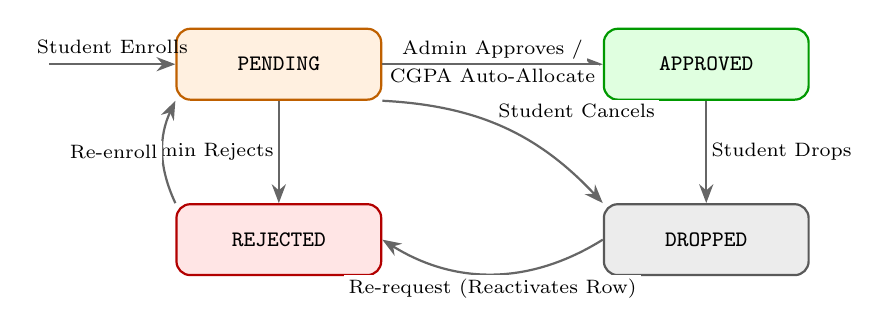
\begin{tikzpicture}[
    node distance=1.4cm and 2.2cm,
    state/.style={rectangle, rounded corners=5pt, draw=blue!70!black, thick, fill=blue!6, minimum width=2.6cm, minimum height=0.9cm, align=center, font=\footnotesize\bfseries},
    edge_lbl/.style={font=\scriptsize, fill=white, inner sep=1.5pt},
    arrow/.style={-{Stealth[length=2.4mm]}, thick, draw=gray!80!black}
]
    \node[state, fill=orange!12, draw=orange!75!black] (pending) {\texttt{PENDING}};
    \node[state, right=2.8cm of pending, fill=green!12, draw=green!60!black] (approved) {\texttt{APPROVED}};
    \node[state, below=1.3cm of pending, fill=red!10, draw=red!70!black] (rejected) {\texttt{REJECTED}};
    \node[state, below=1.3cm of approved, fill=gray!15, draw=gray!70!black] (dropped) {\texttt{DROPPED}};

    \draw[arrow] ([xshift=-1.6cm]pending.west) -- node[above, font=\scriptsize] {Student Enrolls} (pending.west);
    \draw[arrow] (pending) -- node[above, edge_lbl] {Admin Approves /} node[below, edge_lbl] {CGPA Auto-Allocate} (approved);
    \draw[arrow] (pending) -- node[left, edge_lbl] {Admin Rejects} (rejected);
    \draw[arrow] (approved) -- node[right, edge_lbl] {Student Drops} (dropped);
    \draw[arrow, bend left=22] (pending.south east) to node[pos=0.45, above right, edge_lbl] {Student Cancels} (dropped.north west);
    \draw[arrow, bend left=32] (dropped.west) to node[below, edge_lbl] {Re-request (Reactivates Row)} (rejected.east);
    \draw[arrow, bend left=25] (rejected.north west) to node[left, edge_lbl] {Re-enroll} (pending.south west);
\end{tikzpicture}
\caption{Enrollment state transition lifecycle enforcing \texttt{UNIQUE(student\_id, course\_id)}.}
\label{fig:enrollment-lifecycle}
\end{figure}

\subsection{Rules enforced}
\begin{itemize}
  \item Only an active student can request a course, and only an active (not archived) course accepts requests.
  \item Duplicate requests are rejected.
  \item The administrator can open or close the \emph{enrollment period}. While it is closed, students
        cannot request courses; approvals and drops still work. The setting is stored in a small
        \texttt{settings} table created on first use, so \texttt{schema.sql} did not change.
  \item Capacity is checked when a request is approved, so the number of approved students never exceeds
        the course capacity.
  \item Students see and change only their own enrollments; every service method checks the role first.
\end{itemize}

\subsection{Capacity and CGPA-based allocation}
When more students request a course than it has seats, the administrator can run automatic allocation.
Pending students are ranked by CGPA (highest first, ties broken by roll number) and approved until the
course is full. The remaining requests stay pending. The CGPA is computed by \texttt{CgpaCalculator} from
published grades, using the course credits and the assignment weights. Until grades are published, every
CGPA is $0.0$, so allocation falls back to the tie-break order.

\subsection{Timetable clashes and prerequisites}
Our final schema is for a single semester and gives every course a \emph{slot}. A partial unique index
allows only one active course per slot, so two active courses can never clash in time. Because of this
rule, no separate clash check is needed in the enrollment code, and the schema has no prerequisite table.

\subsection{Reports and CSV export}
The service provides four reports for the administrator: enrollment counts per course, course roster,
grade averages per course, and student transcript (percentage and letter grade per course, with the CGPA
in the title). Only \emph{published} grades are used. \texttt{CsvExporter} writes any report table to a CSV
file. The same reports are available from the command line through \texttt{python/reports.py}, which can
also draw a grade-average chart and a bell curve for one course.

\subsection{Usage}
\begin{enumerate}
  \item Run \texttt{bash scripts/setup.sh} to create the database, then \texttt{bash scripts/run.sh}.
  \item As administrator, open \emph{Enrollments} and use the \emph{Enrollment: OPEN/CLOSED} button.
  \item As a student, open \emph{Browse Courses}, search, and press \emph{Enroll}. A clear message is shown
        for errors such as a full course or a closed enrollment period.
  \item As administrator, filter pending requests by course and approve or reject them, or run the allocation.
  \item Students see their courses under \emph{My Courses} and the weekly grid under \emph{Timetable}.
\end{enumerate}

\subsection{Results}
The module is covered by 22 JUnit tests (\texttt{EnrollmentServiceTest}, \texttt{CsvExporterTest} and
\texttt{EnrollmentPeriodAndReportsTest}); the whole project passes 136 Java tests. The profiling results for
the enrollment queries on a database of 10{,}006 students and 50{,}040 enrollments are given in the
profiling section.


\section{Performance Profiling and Query Optimization}
\label{sec:profiling}

\subsection{Profiling Methodology and Experimental Setup}
To evaluate database performance under institutional load, the system was subjected to query profiling on a database populated with 10{,}006 students (10{,}000 generated via \texttt{python/generate\_data.py}), 43 courses, 50{,}040 enrollments, 84 assignments, and 70{,}301 grades.

Profiling was orchestrated by \texttt{python/profile\_queries.py} and executed via \texttt{scripts/profile.sh}. The tool benchmarks the most frequently executed SQL queries (extracted directly from \texttt{EnrollmentDAO} and \texttt{CgpaCalculator}) across 30 repeated runs with a fixed random seed to ensure identical query parameters between runs. Query timings represent raw database execution times in milliseconds, excluding GUI and JDBC overhead.

\subsection{Bottleneck Identification}
Before introducing optimization indexes, \texttt{EXPLAIN QUERY PLAN} revealed extensive full table scans (\texttt{SCAN enrollments}, \texttt{SCAN grades}, \texttt{SCAN students}) on critical paths. The primary bottleneck was the \textbf{Browse Courses} query, which required 146.49\,ms to execute. For each course offering, the query counts active approved enrollments; without an index on \texttt{course\_id} and \texttt{status}, each calculation scanned all 50{,}040 rows in the \texttt{enrollments} table. Because this view is the first screen encountered by students upon logging in, indexing was deemed essential.

\subsection{Index Implementation}
To resolve these bottlenecks without altering the base \texttt{db/schema.sql}, five targeted indexes were specified in \texttt{db/indexes.sql}:
\begin{enumerate}
    \item \texttt{CREATE INDEX idx\_enrollments\_course\_status ON enrollments(course\_id, status);}: Optimizes seat capacity checks, course roster queries, and Browse Courses filtering.
    \item \texttt{CREATE INDEX idx\_enrollments\_status ON enrollments(status);}: Accelerates status aggregations displayed on administrator dashboard cards.
    \item \texttt{CREATE INDEX idx\_grades\_student ON grades(student\_id);}: Enables fast retrieval of individual student grades for transcript generation and CGPA calculation.
    \item \texttt{CREATE INDEX idx\_assignments\_course ON assignments(course\_id);}: Accelerates course-level grade reporting and assignment lookups.
    \item \texttt{CREATE INDEX idx\_students\_name ON students(name COLLATE NOCASE);}: Optimizes case-insensitive student name prefix searches.
\end{enumerate}

Existing unique constraints on \texttt{UNIQUE (student\_id, course\_id)} and \texttt{UNIQUE (assignment\_id, student\_id)} already generate implicit B-tree indexes, so no additional indexes were required for direct student-course or assignment-student lookups.

\subsection{Benchmark Results}
Table~\ref{tab:profiling-results} summarizes average execution times across 30 iterations before and after applying \texttt{db/indexes.sql} and running \texttt{ANALYZE}.

\begin{table}[htbp]
\centering
\small
\begin{tabular}{|l|r|r|r|}
\hline
\textbf{Query Description} & \textbf{Before (ms)} & \textbf{After (ms)} & \textbf{Speed-up} \\ \hline
Seats taken (single course) & 3.122 & 0.059 & 53.0$\times$ \\ \hline
Admin card: count by status & 3.442 & 0.274 & 12.6$\times$ \\ \hline
Admin table: one course + PENDING & 3.717 & 0.806 & 4.6$\times$ \\ \hline
Admin table: all PENDING & 34.019 & 30.478 & 1.1$\times$ \\ \hline
Student: my enrollments & 0.051 & 0.034 & (already indexed) \\ \hline
\textbf{Student: browse courses} & \textbf{146.494} & \textbf{1.983} & \textbf{74.0$\times$} \\ \hline
\textbf{CGPA: grades of one student} & \textbf{2.512} & \textbf{0.025} & \textbf{100.0$\times$} \\ \hline
Report: enrollment counts & 63.052 & 8.785 & 7.2$\times$ \\ \hline
Report: grade averages & 98.840 & 99.633 & none \\ \hline
Admin search: name prefix & 1.017 & 0.175 & 5.8$\times$ \\ \hline
\end{tabular}
\caption{Average query execution times before and after index optimization (SQLite, 10{,}006 students).}
\label{tab:profiling-results}
\end{table}

\subsection{Analysis and Trade-offs}
\begin{itemize}
    \item \textbf{High-Impact Gains:} The Browse Courses query experienced a \textbf{74$\times$ speed-up} (reduced from 146.5\,ms to under 2\,ms). CGPA calculation achieved a \textbf{100$\times$ speed-up} (from 2.5\,ms to 0.025\,ms), allowing instantaneous calculation of student grade point averages during allocation.
    \item \textbf{Unimproved Queries:} The \emph{Grade Averages} report must aggregate all 70{,}301 published grade records to compute class averages; because all rows must be read, index lookups cannot bypass the data scan. Similarly, the \emph{All Pending} query returns thousands of records where execution time is dominated by result set construction and serialization rather than search. The name index only helps prefix searches; a search for text in the middle of a name cannot use an index.
    \item \textbf{Trade-off Assessment:} B-tree indexes introduce marginal overhead on \texttt{INSERT} and \texttt{UPDATE} operations and consume additional disk storage. Because academic course management systems are predominantly read-heavy (frequent course browsing, enrollment checks, and grade reviews compared to course creation), this trade-off is highly beneficial.
\end{itemize}

\subsection{Profiling the Python Report Tool}
We also profiled \texttt{python/reports.py} with \texttt{cProfile} on the 10{,}006-student database
(one run per report). For both reports, about 63--70\% of the profiled time was the SQLite query
itself (\texttt{sqlite3.Connection.execute}); the rest was mostly Python start-up and module imports,
and printing the table was too small to appear among the top entries. The SQL, and therefore its
indexes, remains the right place to optimise. These are single runs, so the 30-run measurements in
Table~\ref{tab:profiling-results} are the more precise ones.


\section{Automated Testing and Verification}
\label{sec:testing}

\subsection{Testing Philosophy and Strategy}
To prevent regressions across collaborative features and guarantee data integrity, the project implements a rigorous dual-layer automated testing strategy combining Java JUnit 5 tests and Python standard library unit tests.

Testing guidelines strictly enforce:
\begin{enumerate}
    \item \textbf{Hermetic Test Isolation:} Database tests operate against temporary or in-memory SQLite instances created from \texttt{db/schema.sql}, preventing test side-effects from polluting \texttt{data/campus.db}.
    \item \textbf{Role-Based Security Verification:} Every dashboard and protected service method is tested against valid and invalid session roles to verify that unauthorized access throws expected security exceptions.
    \item \textbf{Edge Case Coverage:} Validation includes duplicate entity detection, constraint boundary values (e.g., negative course credits, year out-of-range), and transaction rollback on insertion failure.
\end{enumerate}

\subsection{Module-Wise Test Coverage Summary}
Table~\ref{tab:test-coverage-summary} provides a complete breakdown of all \textbf{147 automated tests} (136 Java JUnit 5 tests and 11 Python \texttt{unittest} tests) across the project modules.

\begin{table}[H]
\centering
\small
\begin{tabular}{|p{0.22\linewidth}|p{0.31\linewidth}|r|p{0.25\linewidth}|c|}
\hline
\textbf{Module / Package} & \textbf{Test Classes / Suites} & \textbf{Tests} & \textbf{Primary Verification Scope} & \textbf{Status} \\ \hline
Authentication (\texttt{auth}) & \texttt{AuthServiceTest}, \texttt{LoginFrameTest}, \texttt{PasswordUtilTest}, \texttt{ProfilePanelTest}, \texttt{UserDAOTest} & 42 & PBKDF2 hashing, login state routing, password changes, user CRUD & 42 / 42 Pass \\ \hline
Core \& UI (\texttt{core}) & \texttt{SessionTest}, \texttt{DashboardCardTest} & 11 & Singleton session RBAC checks, KPI metric card state updates & 11 / 11 Pass \\ \hline
Student Management (\texttt{students}) & \texttt{StudentDAOTest}, \texttt{StudentsPanelTest} & 24 & Roll number uniqueness, branch/year bounds, UI filtering \& CRUD & 24 / 24 Pass \\ \hline
Course Catalog \& Faculty (\texttt{catalog}) & \texttt{CatalogDAOTest} & 6 & Active slot uniqueness, capacity rules, faculty assignment & 6 / 6 Pass \\ \hline
Enrollment \& Reports (\texttt{enrollment}) & \texttt{EnrollmentServiceTest}, \texttt{EnrollmentPeriodAndReportsTest}, \texttt{CsvExporterTest} & 22 & Request/approve/drop rules, CGPA auto-allocation, CSV export & 22 / 22 Pass \\ \hline
Grading (\texttt{grading}) & \texttt{GradesPanelTest} & 3 & Enrolled student auto-population, draft vs.\ published grades & 3 / 3 Pass \\ \hline
Role Dashboards (\texttt{dashboard}) & \texttt{AdminDashboardTest}, \texttt{FacultyDashboardTest}, \texttt{StudentDashboardTest} & 28 & Role guards, sidebar card navigation, KPI \& profile wiring & 28 / 28 Pass \\ \hline
Synthetic Data (\texttt{python}) & \texttt{test\_generate\_data.py} & 11 & 10k scale synthesis, Java PBKDF2 parity, FK \& rollback safety & 11 / 11 Pass \\ \hline
\textbf{Total} & \textbf{17 Java Classes + 1 Python Suite} & \textbf{147} & \textbf{End-to-End System Verification} & \textbf{100\% Pass} \\ \hline
\end{tabular}
\caption{Module-wise automated test coverage summary across Java and Python test suites.}
\label{tab:test-coverage-summary}
\end{table}

\subsection{Java Test Suite (JUnit 5)}
All 136 Java tests execute via Maven and pass with zero failures:
\begin{verbatim}
mvn test
Results: Tests run: 136, Failures: 0, Errors: 0, Skipped: 0
\end{verbatim}

\subsection{Python Test Suite (unittest)}
The synthetic student data generator is verified by 11 comprehensive automated tests in \texttt{python/test\_generate\_data.py}:
\begin{itemize}
    \item Validation of cohort generation across sizes: 100, 1{,}000, and 10{,}000 records.
    \item Exact Java PBKDF2-HMAC-SHA256 password hash vector verification.
    \item Uniqueness guarantees for generated usernames, roll numbers, and emails.
    \item Foreign key referential integrity via SQLite \texttt{PRAGMA foreign\_key\_check}.
    \item Database structure integrity via SQLite \texttt{PRAGMA integrity\_check}.
    \item Atomic rollback verification upon injected insertion failures.
    \item Idempotency and dry-run execution checks.
\end{itemize}

The Python suite executes cleanly:
\begin{verbatim}
python -m unittest python/test_generate_data.py
Ran 11 tests in 49.146s -- OK
\end{verbatim}


\section{Conclusion and Future Work}
\label{sec:conclusion}

\subsection{Project Summary}
The Campus Course Management System (Campus CMS) provides a robust, desktop-based academic management platform backed by SQLite and Java Swing. Through clean architectural separation (DAOs, domain models, business services, and tokenized UI components), the system delivers a cohesive, responsive experience for Administrators, Faculty, and Students.

Key achievements delivered across the collaborative development include:
\begin{enumerate}
    \item A modern, token-driven UI design system and responsive role-based dashboards that resolve visual clutter and control clipping.
    \item A deterministic, high-capacity synthetic data generator that reliably synthesizes 10{,}000+ student records with cryptographic password compatibility in approximately 40 seconds.
    \item Complete course management, assignment grading workflows with automated student roster population, and draft/published grade controls.
    \item A resilient enrollment lifecycle featuring capacity tracking, CGPA-based automatic allocation, and CSV report exports.
    \item Empirical query optimization demonstrating up to a 100$\times$ query speed-up on institutional-scale datasets through five targeted indexes.
    \item High software reliability guaranteed by 136 passing JUnit tests and 11 passing Python tests (147 total automated tests).
\end{enumerate}

\subsection{Prioritized Future Work}
Potential extensions for subsequent iterations are prioritized into short-term operational enhancements and long-term architectural evolutions:

\subsubsection{Short-Term Enhancements (High Priority)}
\begin{itemize}
    \item \textbf{Student Online Assignment Submissions:} Expanding the grading module with a dedicated \texttt{submissions} table to support student file uploads, submission timestamps, and late-submission status tracking directly within \texttt{StudentDashboard}.
    \item \textbf{Cursor-Based Table Pagination:} Introducing server-side/DAO pagination (\texttt{LIMIT}/\texttt{OFFSET} or keyset pagination) on administrative tables such as \emph{All Pending Enrollments} and the 10{,}000-student directory to reduce Swing table rendering overhead.
\end{itemize}

\subsubsection{Long-Term Roadmap (Architectural Evolution)}
\begin{itemize}
    \item \textbf{Multi-Semester Scheduling and Prerequisite Graphs:} Extending the relational schema to model multiple academic terms, historical term-by-term GPA progression, and a \texttt{prerequisites} junction table verified during enrollment requests.
    \item \textbf{Clock-Mapped Timetable Clash Detection:} Replacing abstract single-character slot labels with explicit day-of-week and clock-interval schedules to support multi-hour laboratory sessions and fine-grained conflict resolution.
\end{itemize}


\end{document}
